\documentclass[a4paper]{llncs}

\usepackage{amssymb}
\usepackage{amsmath}
\usepackage{graphicx}
\usepackage{epsfig}
\usepackage{subfigure}
\usepackage{listings}
\usepackage{natbib}
\usepackage{verbatim}
\usepackage{enumitem}
\usepackage[utf8]{inputenc}
\usepackage[T1]{fontenc}
\usepackage[hyphens]{url}
\usepackage{listings}
\usepackage[font=small,labelfont=bf]{caption}
\lstset{language=ml}
\lstset{commentstyle=\textit}
\lstset{mathescape=true}
\lstset{backgroundcolor=,rulecolor=}
\lstset{frame=single}
\lstset{breaklines=true}
\lstset{basicstyle=\footnotesize\ttfamily}


\begin{document}

\title{Resource Entity Action: A Generalized Design Pattern for RTS games}

\author{
Mohamed Abbadi\and Francesco Di Giacomo\and Renzo Orsini\and\\
Aske Plaat \and Pieter Spronck \and Giuseppe Maggiore\\
E-mail: \{mabbadi,fdigiacomo,orsini\}@dais.unive.it,
\{a.plaat,p.spronck\}@uvt.nl,
maggiore.g@nhtv.nl
}

\institute{Universit\`a Ca' Foscari DAIS - Computer Science, Venice, Italy \\[1mm]
Tilburg University, Netherlands\\[1mm]
NHTV University of Applied Sciences, Breda, Netherlands\\[1mm]
}

\date{}
\maketitle

\begin{abstract}
In many Real-Time Strategy (RTS) games, players develop an army in real time, then attempt to take out one or more opponents. Despite the existence of basic similarities among the many different RTS games, engines of these games are often built ad hoc, and code re-use among different titles is minimal. We created a design pattern called ``Resource Entity Action'' (REA) that abstracts the basic interactions that entities have with each other in most RTS games. This paper discusses the REA pattern and its language abstraction. We also discuss the implementation in the Casanova game programming language. Our analysis shows that the pattern forms a solid basis for a playable RTS game, and that it achieves considerable gains in terms of lines of code and runtime efficiency. We conclude that the REA pattern is a suitable approach to the implementation of many RTS games. 
\end{abstract}

\section{Introduction}
\label{sec:introduction}
%%%%%%%%%%%%%%%%%%%%%%%%%%%%%%%%%%%%%%%%%%%%%%%%%%%%%%%%%%
% intro.tex
%%%%%%%%%%%%%%%%%%%%%%%%%%%%%%%%%%%%%%%%%%%%%%%%%%%%%%%%%%

%%%%%%%%%%%%%%%%%%%%%%%%%%%%%%%%
%edit
%%%%%%%%%%%%%%%%%%%%%%%%%%%%%%%%
Computer games promise to be the next frontier in entertainment, with game sales being comparable to movie and music sales in 2010 \cite{ESA}. 

This unprecedented market prospects and potential for computer-game diffusion among end-users has created substantial interest in research on principled design techniques and on cost-effective development technologies for game architectures. Our present endeavour makes a step along these directions. 

Making games is an extremely complex business. Games are large pieces of software with many heterogeneous requirements, the two crucial being high quality and high performance \cite{GAME_OPT}. 


%%%%%%%%%%%%%%%%%%%%%%%%%%%%%%%%
%edit
%%%%%%%%%%%%%%%%%%%%%%%%%%%%%%%%
High-quality in games is comprised by two main factors: visual quality and simulation quality. Visual quality in games has made huge leaps forward, and many researchers continuously push the boundaries of real-time rendering towards photorealism. Simulation quality, on the other hand, is often lacking in modern games; game entities often react to the player with little intelligence, input controllers are used in simplistic ways and the logic of game levels is more often than not completely linear. Building a high-quality simulation is very complex in terms of development effort and also results in computationally expensive code. To make matters worse, gameplay and many other aspects of the game are modified (and often even rebuilt from scratch) many times during the course of development. For this reason game architectures require a lot of flexibility.

To manage all this complexity, game developers use a variety of strategies. Object-oriented architectures, components, reactive progamming, etc have all been used with some degree of success for this purpose \cite{COMPONENTS1,GAMEOBJECTS,FRP}. 

In this paper we will present the Casanova language, a language for making games. Casanova offers a mixed declarative/procedural style of programming which has been designed in order to facilitate game development. The basic idea of the language is to require from the developer only and exclusively those aspects of the game code which are specific to the game being developed. The language aims for simplicity and expressive power, and thanks to automated optimizations it is capable of generating code that is much faster than hand-written code and at no effort for the developer. The language offers primitives to cover the development of the game logic, and incorporates the typical processing of a game engine. Also, the language is built around a theoretical model of games with a ``well-formedness'' definition, in order to ensure that game code is always a good model of the simulated virtual world.

In the remainder of the paper we show the Casanova language in action. We begin with a description of the current state of game engines and game programming in Section \ref{sec:background}. In Section \ref{sec:model} we define our model of games. We describe the Casanova language in Section \ref{sec:casanova}.  We show an example of Casanova in action, and also how we have rewritten the game logic of an official XNA sample from Microsoft \cite{XNA_SAMPLES} in Casanova with far less code and higher runtime performance in Section \ref{sec:case_study}. In Section \ref{sec:conclusions} we discuss our results and some future work.


\section{Essential elements of RTS games}
\label{sec:the_problem}
RTS are a variation of strategy games where two or more players achieve specific (often conflicting) objectives by performing actions simultaneously in real time. The typical elements which arise from this genre are \textit{units} (characters, armies), \textit{buildings}, \textit{resources} and \textit{battle statistics}. Players command units to perform different types of actions. These actions can affect several entities in the game world.

Units and buildings are the entities that players control to achieve their objectives. Units usually fight or harvest resources, while buildings may be used to create new units or research upgrades. Resources are gathered from the playing field and fuel the economy of the game entities. Battle statistics determine the offensive and defensive abilities of units in a fight. This taxonomy of the elements of an RTS game can be applied successfully to multiple games: Starcraft, C\&C, and Age of Empires all feature units, buildings, resources, and battle statistics, amongst other elements.

In order to arrive at our design pattern we will now apply a simplification. Battle statistics can be interpreted as \textit{resources}, as for instance: ``the life of a unit is the cost for killing it, payable in attack power.'' We can also merge units and buildings together into a new category called \textit{entities}. This leads us to a simpler view of an RTS as a game that is based on Resources, Entities and Actions:

\begin{enumerate}
\item Resources: numerical values in the battle and economic system of the game. In this group we find the \textit{attack}, \textit{defense}, and \textit{life} patterns of entities. Resources also cover building materials and costs of production, deployment of units, development of new weapons, etc. (Resources are scalars.)
\item Entities: container for resources. They have physical properties and, as for the game logic, the difference among them lies only in the interactions. These interactions take place with resource exchanges through the actions. (Entities are vectors.)
\item Actions: resource flow among entities. Our model can be viewed as a directed weighted graph where the nodes are the entities, the weights are the amounts of exchanged resources, and the edges are the actions, that is, the elements which connect entities to one another. (Actions are transformation matrices.)
\end{enumerate}

Next, we discuss how we model Resources, Entities and Actions. 

\section{The REA design pattern}
\label{sec:the_idea}
In this section we will define a model for an algebra to show that the REA (Resource Entity Action) model can be reduced to a problem of linear algebra. We then show how games that use this model can be further simplified by linguistic constructs.

\subsection{Action algebra}

An action consists of a transfer of resources from a source entity to one or more target entities. We require that each entity has a resource vector, which contains the current amount of resources of the entity. The resource vector is sparse, since most actions involve only few resource types. An action is expressed by a transformation matrix $A$.

Consider a set of target entities $T = \left\lbrace t_{1},t_{2},...,t_{n}\right\rbrace$, which are the targets of the action, and a source entity $e$. Each entity $t_{i}$ (including the source entity type) has a resource vector
$\mathbf{r_{i}}=\left(r_{i_{1}},r_{i_{2}},...,r_{i_{m}} \right)$. The source entity also has a transformation matrix $A$ of size $m \times m$, which defines the interactions between all the resources of the source entity and all the resources of the target entities. We also consider an integrator $dt$ which contains the time difference between the current frame and the previous one. We then compute $\mathbf{w_{e}} = \left(  w_{e_{1}},w_{e_{2}},...,w_{e_{m}} \right) = \mathbf{r_{s}} \times A \cdot dt$. From the definition of matrix multiplication, it immediately follows that each component of $ \mathbf{w_{e}}$ represents how a resource will change by applying the effect of all the other resources to it. We compute the vector $\mathbf{r'_{i}} = \mathbf{r_{i}} + \mathbf{w_{e}} \; \forall e_{i} \in E$
which replaces the resource vector in each target entity.

For instance, consider the action of a spaceship (entity) using laser to damage (resource) an enemy spaceship (entity). This involves a  vector resource of two elements: laser and life points. The action must transfer laser points to subtract from the enemy life points. Suppose that the vector resource of the targeting ship is $r_{s} = (20,500)$ and the vector resource of the targeted ship is $r_{t} = (15,1000)$. Let the transformation matrix be
$A =
\begin{bmatrix}
0 & -1\\
0 & 0\\
\end{bmatrix}
$
which means that the source entity will reduce the life of the target by the number of its laser points.
Thus $w_{e} = r_{s} \times A  \cdot dt = (20,500) \times A  \cdot dt = (0,-20) \cdot dt$. At this point, assuming $dt = 1$ second, we have $r'_{t} = r_{t} + w_{e} = (20,1000) + (0,-20) \cdot dt = (20,980)$.

\subsection{A declarative language extension}

We now describe a language extension that implements the REA design pattern and its associated algebra for the Casanova game programming language \citep{Casanova}. The language extension is purely declarative. Its semantics are described using the SQL query language, which has the advantage of familiarity to most programmers.

%Implementing the action algebra is done using an abstract class which contains an abstract method which performs the action. Each action is a class which extends the previous abstract class and implements the abstract method. This method will fetch the world looking for the information needed to find what entities are affected by the action execution. Each entity of the game will have a collection of actions it can perform, automatically run by Casanova.

To identify the set of target entities $T$ given a source entity and its action, we create a new type definition called \textit{action}. An action is a declarative construct which is used to describe not only the resource exchange between entities, but also what kinds of entities participate in the exchange. The resource exchange is based on \textit{transfers} (Add, Subtract, and Set), while the target determination is based on \textit{predicates}: we filter the game world entities depending on their types, attributes and radius (specifying the distance beyond which the action is not applied). Some actions, called threshold actions, are not continuous and make use of special predicates to delay the execution (Output) until certain conditions are met.

Using actions it is possible to specify an exchange of resources in a fully declarative manner, so that the developer does not have to rewrite similar pieces of code ad hoc for each action. 

\section{Action syntax and semantics}
\label{sec:details}
\begin{itemize}
\item Static analysis technique to detect dependencies.
\item We use these dependencies to generate data structure for scheduling interrupted rules.
	\begin{itemize}
	\item Each entity maintains a list of entities depending on it, and a list of inactive rules.
	\item Maintaining the list according to the dynamics of entities in the game (creation, update, and removal).
	\end{itemize}
\item To what extent a game can benefit from such an optimization? Game state changing too fast. Optimization data structures create overhead which surpass the performance gained by our scheduling.
\item Dynamic analysis technique to detect the update frequency.
\item Rules that update too often will not benefit from our optimization and are not included.
\item The choice of the update threshold depends on the data structure we are using for the optimization.
\item Further optimization: data structures can be stored in the world instead of locally into entities for better cache coherence.
\end{itemize}

A problem that arises from the use of some of these operators is that of \textit{busy waiting}. For instance, the healer behaviour requires that he waits for a guard to ask for healing before leaving the guard post. To describe this behaviour we must continuously check if a wounded guard is nearby. The overhead of this operation is minimum for just one guard, but for a greater amount of guards this can seriously affect the game performance, since it is required that the healer checks if any guard is close enough at every game frame. This observation can be generalized for rules which wait for a condition on values of the game state altered by other rules. Consider the following example in Casanova 2:

\begin{lstlisting}[mathescape]
entity E = {
   A : int
	
   rule A = //rule $r_{1}$
      wait 1.0
      yield A + 1
   rule A = //rule $r_{2}$
      wait A % 2 = 0
      //execute rule body $b_{2}$
   rule A = //rule $r_{3}$
      wait A % 5 = 0
      //execute rule body $b_{3}$
   rule A = //rule $r_{4}$
      wait A % 10 = 0
      //execute rule body $b_{4}$
      
   Create() = {A = 0}		
}
\end{lstlisting}
In the snippet of code shown above, rule $r_{1}$ increments the field A by 1 every second. Rules $r_{2}$, $r_{3}$, and $r_{4}$ wait until A is multiple of respectively 2, 5, and 10 before executing the rest of their bodies. If we assume that running rule bodies $b_{2}$, $b_{3}$, and $b_{4}$ take 0.5 seconds, and we consider a time span of 12 seconds, then $r_{2}$ will be inactive for 10 seconds and run for 2 seconds, $r_{3}$ will be inactive for 11 seconds and run for 1 seconds, and $r_{4}$ will be inactive for 11.5 seconds and active for 0.5 seconds. This comparison is shown in Figure \ref{fig:s4f1}. The time amount in the light grey bars is spent by rules by busy waiting, since in that time interval they keep checking the synchronization condition. We observe that the reactivation of a rule body execution depends only on a change on the fields used in the boolean expression of the \texttt{wait} operator, and this change can only be performed by other active rules (in our example only $r_{1}$, but in a more general case there could be more than one rule acting on the same field). From this consideration we argue that we can make waiting dependent on the game state rather than on the rule state.

\begin{figure}
	\centering
	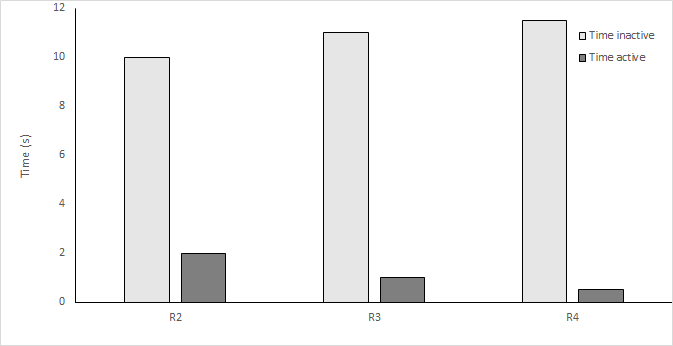
\includegraphics[scale=0.5]{Image/wait_chart}
	\caption{Chart showing the time spent by inactive and active rules}
	\label{fig:s4f1}
\end{figure}

Given that the evaluation of a waiting condition changes only when at least one of the fields affecting it has changed, we keep track of all rules waiting for a change on that field (this can be done statically by examining the expression of a \texttt{wait} operator). When a rule evaluates the condition of a \texttt{wait} operator, if the condition evaluates to \texttt{false}, it is suspended. When another rule changes a field, it resumes any suspended rules with that field. Suspended rules evaluate again the \texttt{wait} conditions. Those which evaluate to \texttt{false} remain suspended, those which evaluate to \texttt{true} become active again and proceed with their execution.

The other operators affected by busy waiting are the concurrency operator and the pre-emption operator (the parallel operator keeps executing its code continuously and it does not wait for any condition itself, although its body can contain other operators that do).

\section{Case study}
\label{sec:evaluation}
We now present an RTS game we used as a case study, created with Casanova, and the benchmarks that test the action implementation. In the game players must conquer a star system made up of various planets. Each planet builds fleets which are used to fight the fleets of the other players and to conquer more planets. A planet is conquered when a fleet of a player is near it and no other enemy fleet is defending it.

\subsection{Case study}

Three actions are required in this game: The first action, called \texttt{Fight Action}, defines how a fleet fights enemy fleets in range. The fight action subtracts $0.5 \cdot dt$ \texttt{life} points from the in-range enemy fleet during every frame (action tick).

\begin{lstlisting}[language=Caml]
Fleet = {Position: Rule Vector2;FightAction: FightAction;Owner: Ref Player;Life: Var float32;Fight: FightAction }
\end{lstlisting}

The Fight Action is defined as follows:

\begin{lstlisting}[language=sql]
FightAction = TARGET Fleet; RESTRICTION Owner <> Owner; RADIUS 150.0; TRANSFER CONSTANT Life - 0.5;
\end{lstlisting}

The target is an entity of which the type is \textbf{Fleet}. The condition to execute the action is that the fleet must be an enemy (i.e., not the player). The \texttt{attack range} is 150 units of distance. 0.5 \texttt{life} points are subtracted for every attack.

The second action is called \texttt{BuildAction}. It allows a planet to create a ship. In order to build a ship, a planet must gather 10 mineral units. Each planet has a field called \texttt{GatherSpeed} which determines how fast it gathers minerals. Every tick the planet's mineral stash is increased by this amount. This action is a threshold action where the threshold value is the minerals of the planet. As soon as the threshold value is reached, we set the field \texttt{NewFleet} to TRUE (it is used by the engine to create a new fleet), and \texttt{Minerals} to 0 to reset the counter. The planet and its actions are:

\begin{lstlisting}[language=Caml]
Planet = {Position: Vector2;Owner: Rule Ref Player;NewFleet: Rule bool;BuildAction:BuildAction;EnemyOrbitingFleetsAction : EnemyOrbitingFleetsAction;GatherSpeed: float32;Minerals: Var float32 }
\end{lstlisting}

\begin{lstlisting}[language=sql]
BuildAction =
TARGET Self; TRANSFER CONSTANT Minerals + GatherSpeed; THRESHOLD Minerals 10.0; OUTPUT NewFleet := true; OUTPUT Minerals := 0.0
\end{lstlisting}

A Casanova rule is appointed to read the value of NewFleet and, when it is true, to spawn a new fleet.

The third action is required to check if a planet can be conquered by a fleet. A fleet can conquer a planet if there is no enemy fleet near it and if it is sufficiently close. Thus the action definition is the following:

\begin{lstlisting}[language=sql]
EnemyOrbitingFleetsAction =
TARGET Fleet; RESTRICTION Owner Not Eq Owner; RADIUS 25.0; INSERT Owner -> EnemyOrbitingFleets
\end{lstlisting}

The action will add an enemy fleet close enough to change the owner of the planet.

%Even the concept of drawing lasers can be implemented using the INSERT clause simply adding it to \texttt{FightAction} which inserts in a list all the targeted ships positions. In this way we can draw a laser from the source position to the target position. We omit this aspect for brevity.

\subsection{Evaluation}

We evaluated the performance of our approach with the case study, and two extra examples: an asteroid shooter, and an expanded version of the case study with more complex rules. All were implemented in Casanova. Table \ref{tab:code_length} shows a code length comparison between the REA implementation and standard Casanova rules for all three.

We note that in games with basic dynamics the code saving is low, due to the fact that there are few repeated patterns. The advantage of using REA becomes evident in a game with actions involving many types of targets, such as the expanded case study. Furthermore, we managed to drastically increase the performance of the game logic: as Figure \ref{fps_chart} shows, using REA (labeled ``with actions'') results in a speedup factor of 6 to 25, due to automated optimizations in the query evaluation. We also note that our implementation is flexible and general since it is possible to use actions to express a behaviour, such as a projectile collision, which is outside the domain of RTS games and traditional resource-based systems.

\begin{table}
\centering
\caption{CS (case study), Asteroid Shooter and Expanded CS code length}
\label{tab:code_length}
\begin{tabular}
{|l|c|c|c|c|c|c|}
\hline
& Game Entities & Rules & Actions & Total\\
\hline
\textit{CS with REA} & 41 & 71 & 19 & 131\\
\hline
\textit{CS without REA} & 40 & 90 & 0 & 130\\
\hline
\textit{Asteroid shooter with REA} & 33 & 33 & 6 & 72\\
\hline
\textit{Asteroid Shooter without REA} & 34 & 44 & 0 & 78\\
\hline
\textit{Extended CS with REA} & 135 & 138 & 40 & 313\\
\hline
\textit{Extended CS without REA} & 135 & 328 & 0 & 463\\
\hline
\end{tabular}
\end{table}
\begin{figure}
\centering
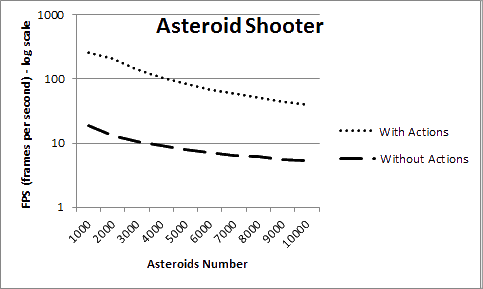
\includegraphics[scale=0.7]{Shooter.png}
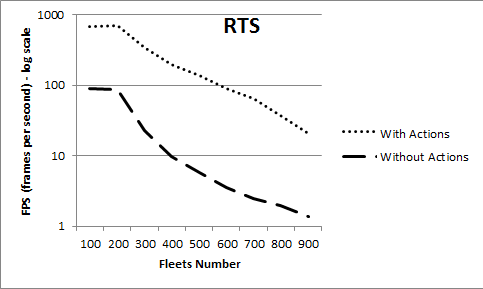
\includegraphics[scale=0.7]{RTS.png}
\caption{Frame rate as a function of numbers of entities.}
\label{fps_chart}
\end{figure} 

%\section{Comparison with related systems}
%\label{sec:related_work}
%%----------------------------------------------------------------------------
%  related_work.tex 
%----------------------------------------------------------------------------

\subsubsection{Region-based memory management}
Tofte and Talpin \cite{8_7} present an inference system for classifying all allocated data of a program into regions and deducing a safe lifetime for each region, which enables provably memory-safe implementations of ML-like languages with-out a garbage collector. Crary et al.'s Capability Calculus \cite{8_6} extends this work by allowing explicit region allocation and deletes, while making sure that all data accesses to a region happen during its lifetime. The commonality of these systems is that only regions are treated linearly; all other objects are allocated within regions and have types akin to guarded types. Regions are not first-class values and cannot be stored in data structures.

\subsubsection{Linear type systems}
Starting with Wadler \cite{8_5}, linear types systems have been used in purely functional languages to enforce single threading on the state of the world or to implement operations like array updating without the cost of a full copy. Linear type systems enable resource management at the granularity of a single object. Every use of an object of linear type consumes the object, leading to a programming style where linear objects are threaded through the computation. Wadler's let! construct, or its variations, can be used to give a temporary nonlinear type to an object of linear type. Walker and Watkins \cite{8_8} study a type system with three kinds of objects: linear, reference counted, and region allocated. The kind of an object is fixed at allocation without a means to change kind. They provide let! only for regions.

\subsubsection{Lighweight static capabilities}
Static capabilities have been implemented by Kiselyov et al. \cite{5_3} in a lightweight fashion in modern functional languages such as OcaML and Haskell. They propose a "style" of programming with three ingredients:
\begin{itemize}
\item A compact kernel of trust that is specific  to the problem domain.
\item Unique names (capabilities) that confer rights and certify properties, so as to extend the trust from the kernel to the rest of the application.
\item Static (type) proxies for dynamic values.
\end{itemize}
The requirements imposed on the host language to implement this style are an expressive core language, higher-rank polymorphism and phantom types. Capabilities are represented as types; safety conditions are stored in types as in dependent-type programming. If a program type-checks, then the type system and the kernel of trust together verify that the safety conditions hold in any run of the program. In most cases, this static assurance costs us no run-time overhead.

\subsubsection{Lightweight Monadic Regions}
Kiselyov et al. \cite{5_1} also build a library that statically ensures the safe use of resources such as file handles. They statically prevent accessing an already closed handle or forgetting to close it. The libraries can be trivially extended to other resources such as database connections and graphic contexts. Their library supports region polymorphism and implicit region subtyping, along with higher-order functions, mutable state, recursion, and run-time exceptions. A program may allocate arbitrarily many resources and dispose of them in any order, not necessarily LIFO. These monadic regions are implemented in Haskell as monad transformers. For contrast, the authors also implement a Haskell library for manual resource management, where deallocation is explicit and safety is assured by a form of linear types. The linear typing is implemented in Haskell with the help of phantom types and a parameterized monad to statically track the type-state of resources.

\subsubsection{Strongly Typed Memory Areas}
Jones et al. \cite{5_4} discuss how to make Haskell suitable for systems programming tasks -including device driver and operating system construction. As a result of some gaps in functionality it often becomes necessary either to code some non-trivial components in more traditional but unsafe languages like C or assembler, or else to adopt aspects of the foreign function interface that compromise on strong typing and type safety. Some of these gaps may be filled by extending a Haskell-like language with facilities for working directly with low-level, memory-based data structures. The authors designed and implemented language features that allow programmers to de?ne strongly typed, high-level views, comparable to programming with algebraic datatypes, on the underlying bitdata structures. A critical detail in making this work is the ability to specify bitlevel layout and representation information precisely and explicitly; this is important because the encodings and representations that are used for bitdata are often determined by third-party speci?cations and standards that must be carefully followed by application programmers and language implementations.


\section{Conclusions}
\label{sec:conclusions}
%% Changed by PS, April 4, 2014.

\section{Future work}
\label{sec:future_work}
The Casanova 2 language is capable of implementing usable and quite complex games. The language, while usable, is currently still in development as it misses a few features. In particular, support for multiplayer games is at this moment lacking. We believe that the existing mechanisms for handling time offered by Casanova 2 could be augmented with relatively little effort in order to greatly simplify the hard task of building multiplayer games. This is part of future work, that we are currently engaging in. We are also doing usability studies using students from various disciplines and backgrounds.

The high level view of the game that the Casanova 2 compiler provides can be exploited in order to improve the programmer experience. This means that we could use tools for code analysis (such as abstract interpretation \cite{nielson1999principles} or type system extensions) in order to better understand the game being built, and to help with correctness analysis, performance analysis, or even optimization.


%\subsection{User study}
%We wish to perform an in-depth user study for Casanova 2 to improve usability in the development process. We have already performed a partial (and quite promising) small user study which we will extend and complete.


%We have performed the following test: we gathered a group of students of game programming and a group of students of game design. We gave them a series of Casanova 2 samples, printed on paper. Each student had to guess the functionality of each sample, and sketch a screen-shot. Furthermore, each student also provided some additional feedback on the language.

%The samples were: (\textit{i}) a string of text moved around the screen with the keyboard, (\textit{ii}) a string of text that moves along a predefined path automatically, and (\textit{iii}) an asteroid shooter.

%Eleven (over a total of thirteen) students understood the samples completely, both drawing the screen-shots and explaining the dynamics of the game correctly. Two students were lost on the syntactic differences between Casanova 2 and the more familiar C-like syntax. The direct feedback was mostly centred around a series of common observations, which are reported in Table \ref{students_feedback}. For each observation, the table reports how many times we encountered it.

%\begin{table}[!t]
%% increase table row spacing, adjust to taste
%\renewcommand{\arraystretch}{1.3}
% if using array.sty, it might be a good idea to tweak the value of
% \extrarowheight as needed to properly center the text within the cells

%\caption{Feedback from students}
%\label{students_feedback}
%\centering

%% Some packages, such as MDW tools, offer better commands for making tables
%% than the plain LaTeX2e tabular which is used here.
%\begin{tabular}{|c||c|}
%\hline
%Syntax is unfamiliar at first & 3\\
%\hline
%Syntax is clear & 8\\
%\hline
%Indentation instead of parentheses is a downside & 2\\
%\hline
%List processing with queries is very effective & 1\\
%\hline
%Rules are a good abstraction for games & 2\\
%\hline
%\end{tabular}
%\end{table}

%We also built a significantly bigger sample, which we asked only three students to study. The sample is a checkpoint-based RTS (see Figure \ref{RTS game} for a screenshot). All students correctly identified the game mechanics, and provided some additional feedback. Most of this feedback overlaps with that obtained for the samples, but some new observations emerge. Arguably, some patterns become visible only with larger samples:
%\begin{itemize}
%\item \texttt{wait} and \texttt{when} are very powerful
%\item Multiple rules on the same field are very powerful
%\item Multiple rules on the same field may lead to behaviours that are complex to understand
%\end{itemize}


\section{Conclusions}
\label{sec:conclusions}

Casanova 2, a language specifically designed for building computer games, may offer a solution for the high development costs of games. The goal of Casanova 2 is to reduce the effort and complexities associated with building games. Casanova 2 manages the game world through entities and rules, and offers constructs (wait and yield) to deal with the run-time dynamics. As shown by the benchmarks in Section \ref{sec:evaluation}, we believe that we have taken a significant step towards reaching these goals. In fact, we achieved at the same time very good performance and simplicity, thereby empowering developers with limited resources. 


\bibliographystyle{plain}
\bibliography{Sections/reference}

\end{document} 